\chapter{Methodology}\label{ch:A}
\hspace{10mm}This chapter introduces analysis of marketplaces, creating UI/UX design,
functionality for specialists and functionality for clients.


‘Asar’  is a mobile application which helps to make life better. In other words, it helps clients to find specialists by their purpose. Also helps specialists to take orders. Having a united source of specialists and clients makes the process of communication easier.


‘Asar’ consists of design,  mobile application, and firebase as back-end.

\section{Stack of technologies}
\hspace{7mm}Technologies which were used during the development of application shown below. \newline
For mobile development was used:
\begin{itemize}
    \item \textbf{Xcode} - is a MacOS software for app development created by Apple. It is the only technique to develop iOS and other Apple OS apps that is officially supported. For designing iOS apps, Xcode has a lot of tools and perks. It comes with tools to assist developers at every stage of the engineering process.
    \item \textbf{Swift} - is a programming language for iOS, iPadOS, macOS, tvOS, and watchOS that is both strong and attractive. Swift code is interactive and enjoyable to write, with succinct yet expressive syntax and modern developer features. Swift code is designed to be safe while simultaneously producing software that runs quickly. 
    \item \textbf{UIKit} -  (user interface kit) is a package of assets that includes design elements such as UI components and styles. Users interact with UI components, which transmit meaning and offer functionality. Input forms, widgets, and navigation menus are examples of UI components.
    \item \textbf{SwiftGen} - is a tool that generates Swift code for your project's resources, making them type-safe. SwiftGen uses auto-generated Swift code to organize and manage your resources.
\end{itemize}
For UI/UX was used: 
\begin{itemize}
    \item \textbf{Figma} - is one of the most innovative graphics editing apps now sweeping the creative world. The fact that it is free to use is what makes it so appealing.
    \item \textbf{Miro} - is an online collaborative whiteboard tool that allows dispersed teams to collaborate efficiently on everything from brainstorming to planning and managing agile workflows.
\end{itemize}
For back-end was used:
\begin{itemize}
    \item \textbf{Firebase} - is a Backend-as-a-Service (Baas). It offers a variety of tools and services to assist developers create high-quality apps, expand their user base, and make money. It is based on Google's technology.
\end{itemize}
For analysis was used:
\begin{itemize}
    \item \textbf{Excel} - is a spreadsheet program that is included in the Microsoft Office Suite. Worksheets (spreadsheets) are created in MS Excel to store and arrange data in a table format.
\end{itemize}
For management was used: 
\begin{itemize}
    \item \textbf{Trello} -  is a team project management program that allows you to track team projects, highlight tasks in progress, see who they're allocated to, and track progress toward completion.
\end{itemize}
\section{Analytical surveys and observations}
\hspace{7mm}Before entering the sphere, made an analysis on market research of some spheres, and by results were chosen exactly this place for connecting specialists and customers. On alternatives in the kz market , there are only 2 applications that are having similar logic to our project. Those applications were analyzed to find drawbacks of why people still don’t use them or what may push away potential customers and specialists. 
\begin{figure}[H]
    \centering
    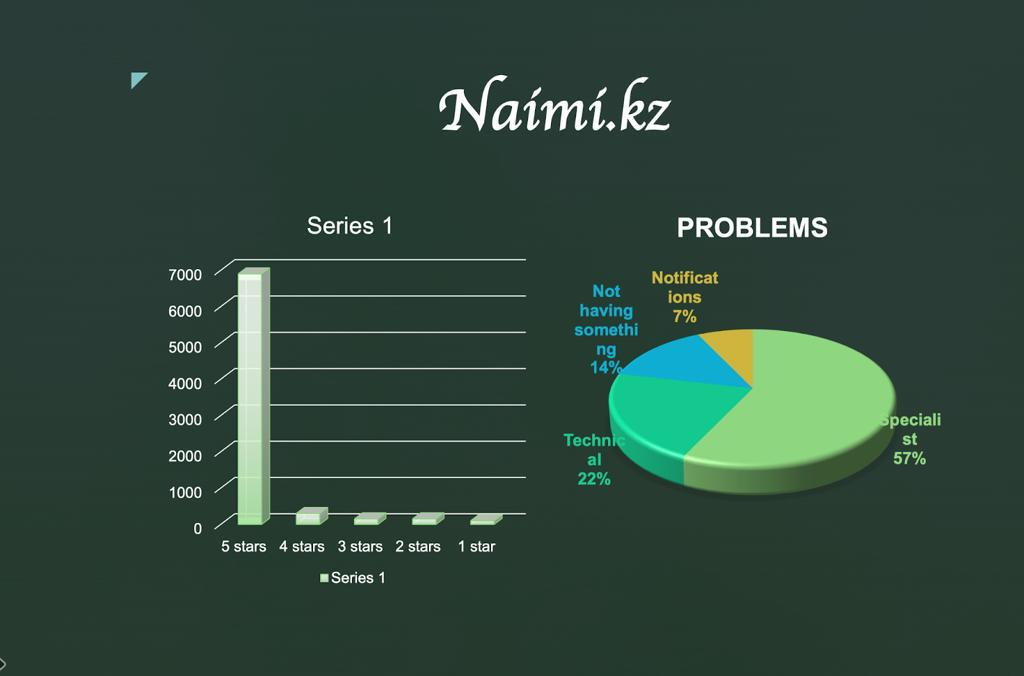
\includegraphics[scale=0.45]{images/naimikz.png}
    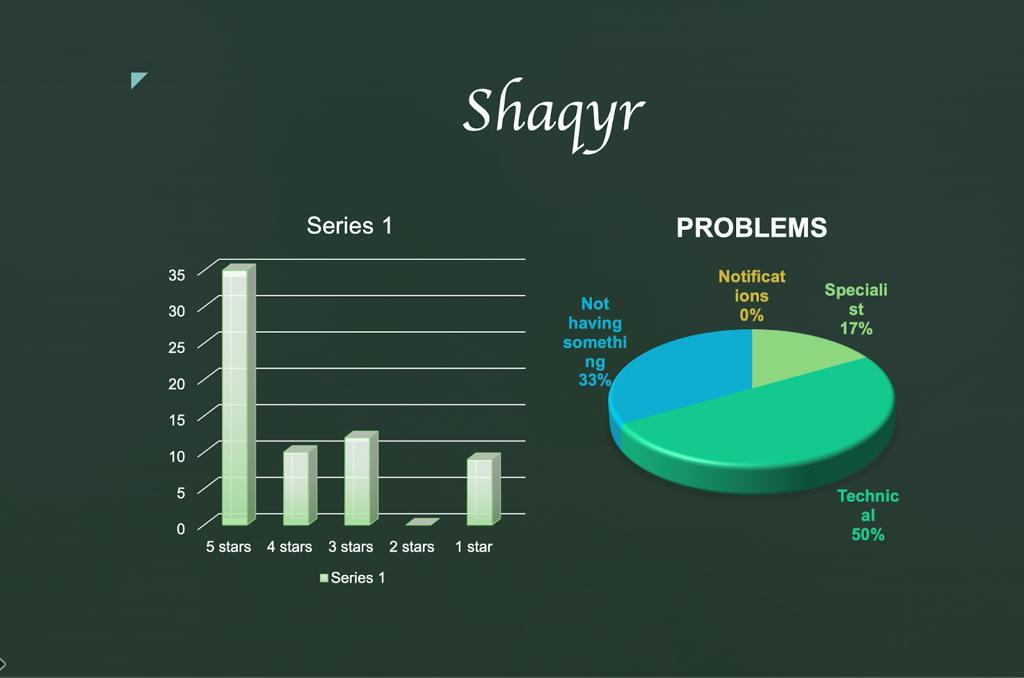
\includegraphics[scale=0.45]{images/shaqyr.png}
\end{figure}
After finding out that the main drawback is specialists , we made an analysis on how to find best specialists and excluding resume of work experience , what questions are most likely should be asked to find more qualified applicants. One of the most important parts is to know the opinions of potential customers and users about the ideas we are inventing . Here is a survey on mostly students to understand how their group of human beings will react to this kind of application and also considering their interests also included in the survey. By next our analytic made a survey for specialists , to take the needed and relevant questions. The survey was made based on important qualities that specialists must need.
\begin{figure}[H]
    \centering
    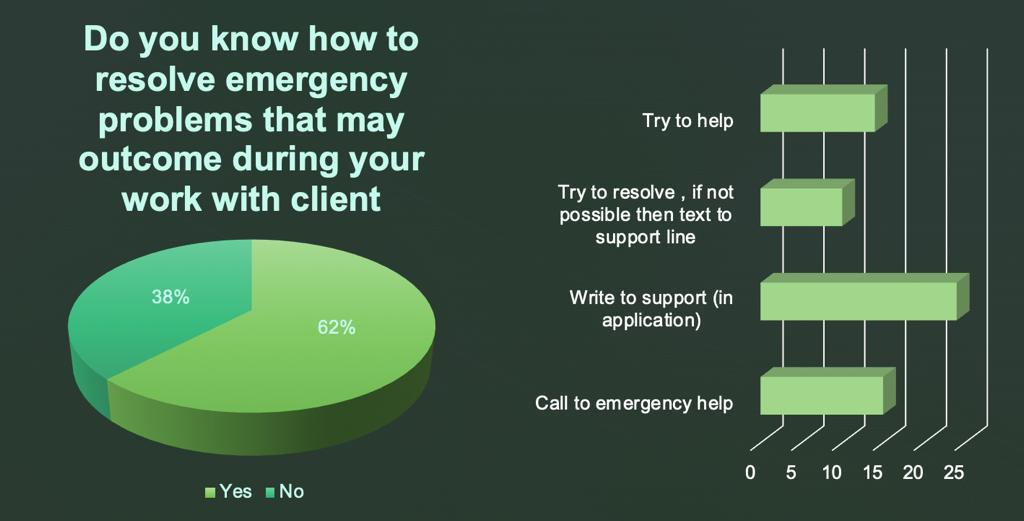
\includegraphics[scale=0.45]{images/analysis.png}
    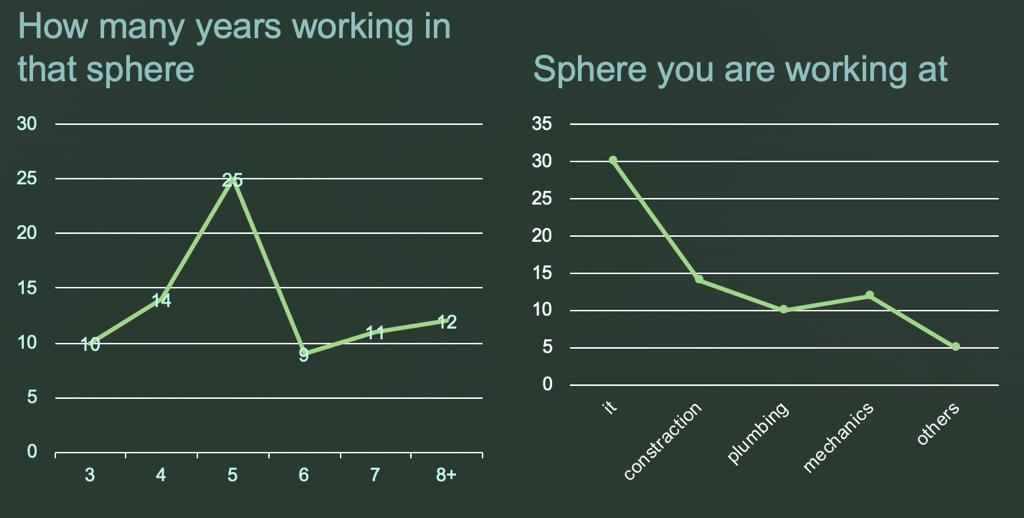
\includegraphics[scale=0.45]{images/analysis1.png}
\end{figure}
Analytical part to find the needs of the customers and finding interests of specialist was used google docs and excel to sort all the answers and see the chart with results for easy analysis.
\begin{figure}[H]
    \centering
    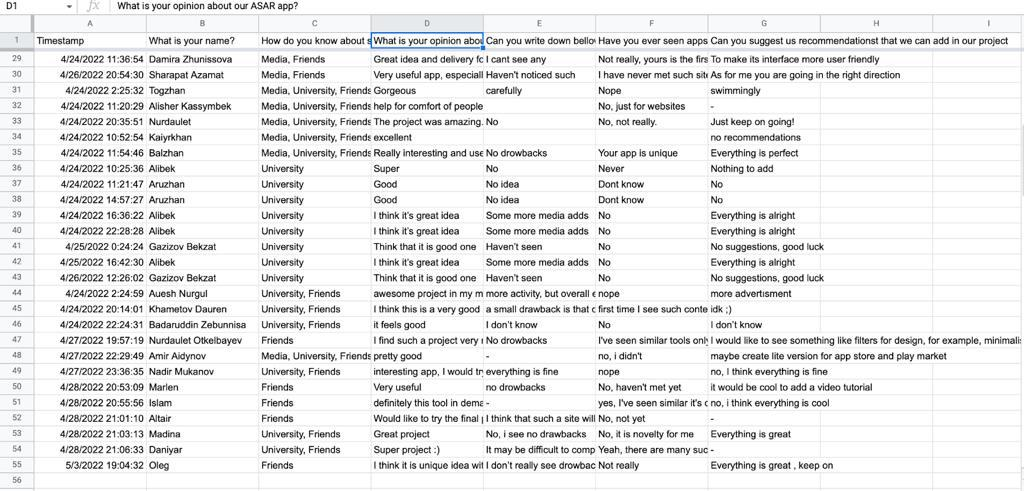
\includegraphics[scale=0.45]{images/excelform.png}
\end{figure}
\section{UI/UX design}


The design part started with learning the Ios platform, studying the pains of customers and solving their problems. After researching, intensively started processing the moodboard.
\begin{figure}[H]
    \centering
    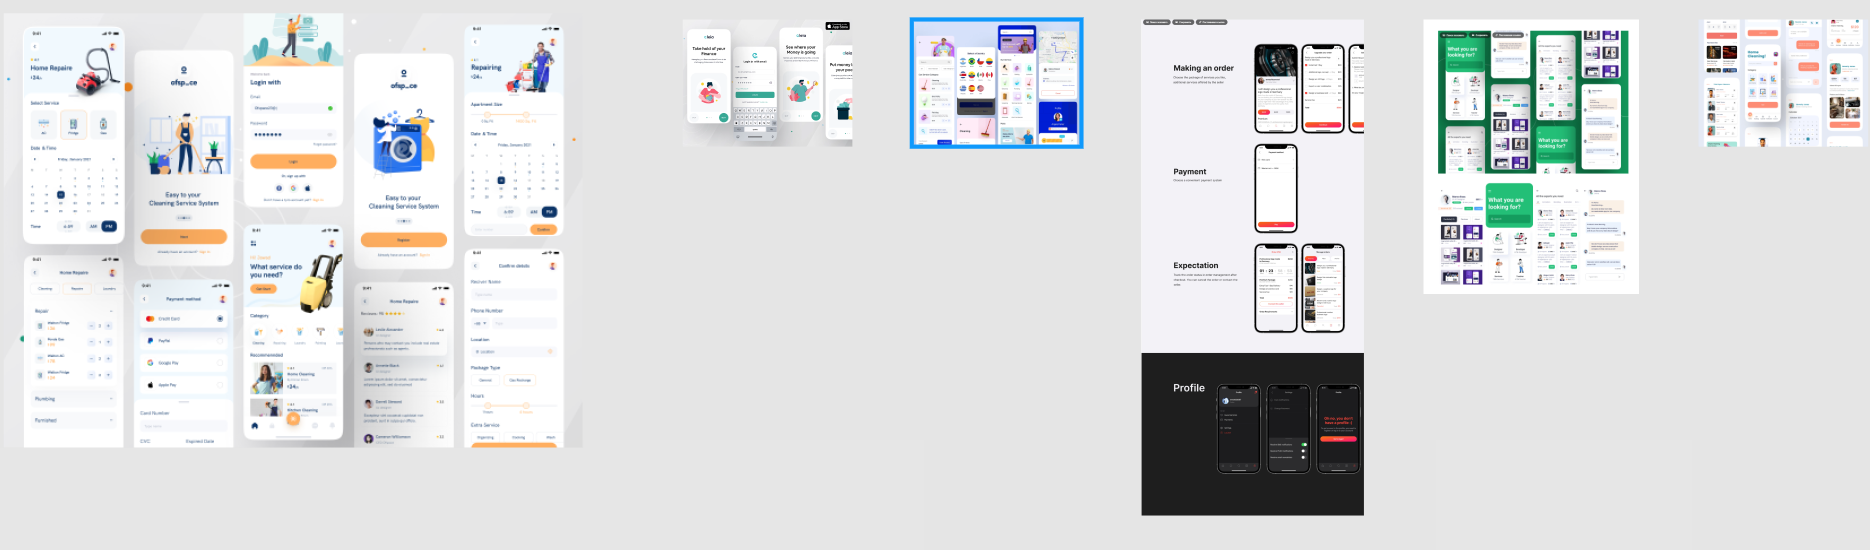
\includegraphics[scale=0.50]{images/design5.png}
\end{figure}
One of the most important parts of designing was the UX part. Cause, User Experience is user perception and response of user results. \newline
UX design of onboarding page:
\begin{figure}[H]
    \centering
    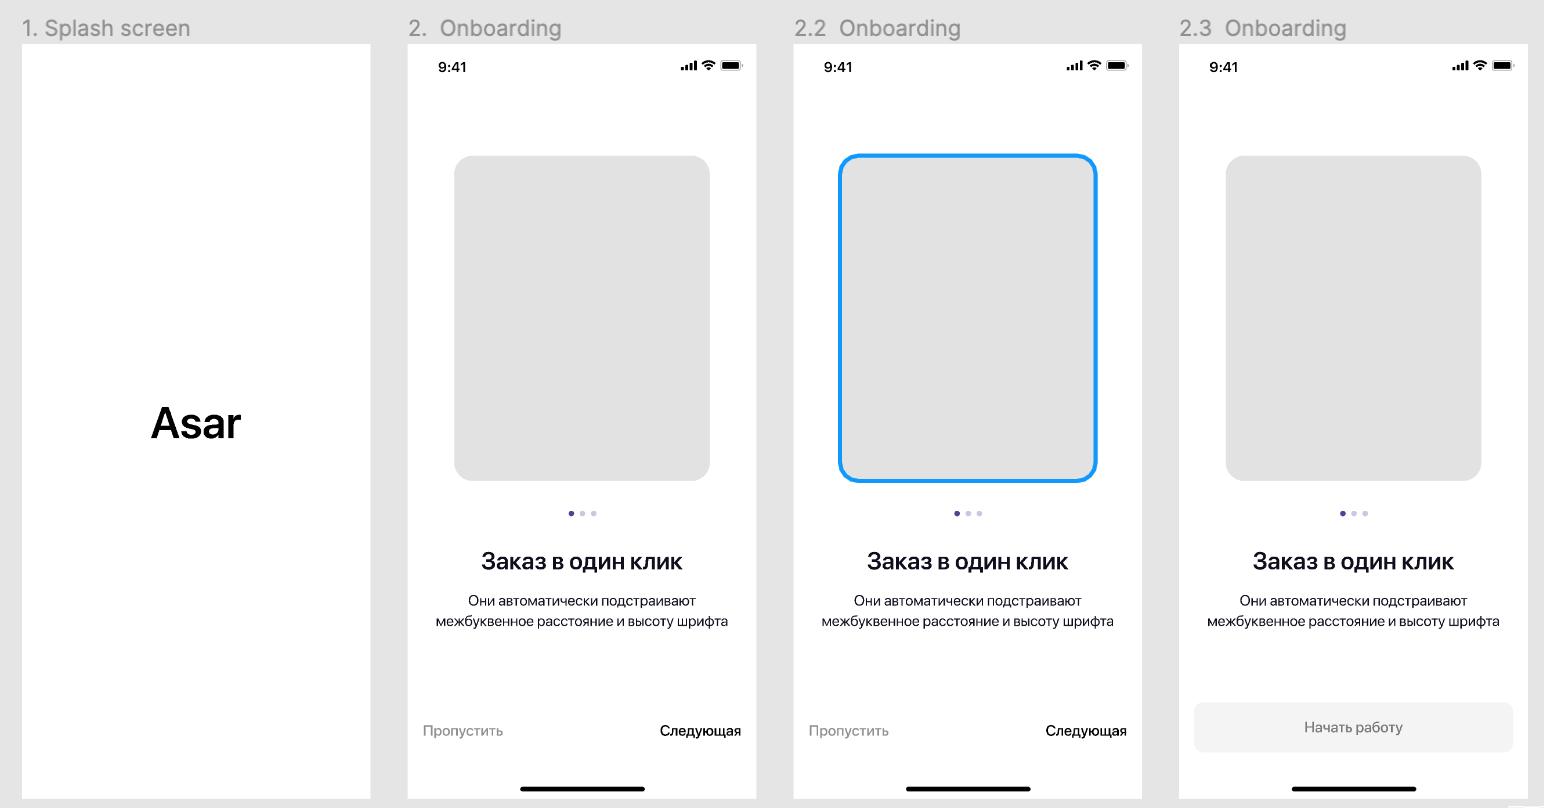
\includegraphics[scale=0.60]{images/design2.png}
\end{figure}
UX design of login/registration page:
\begin{figure}[H]
    \centering
    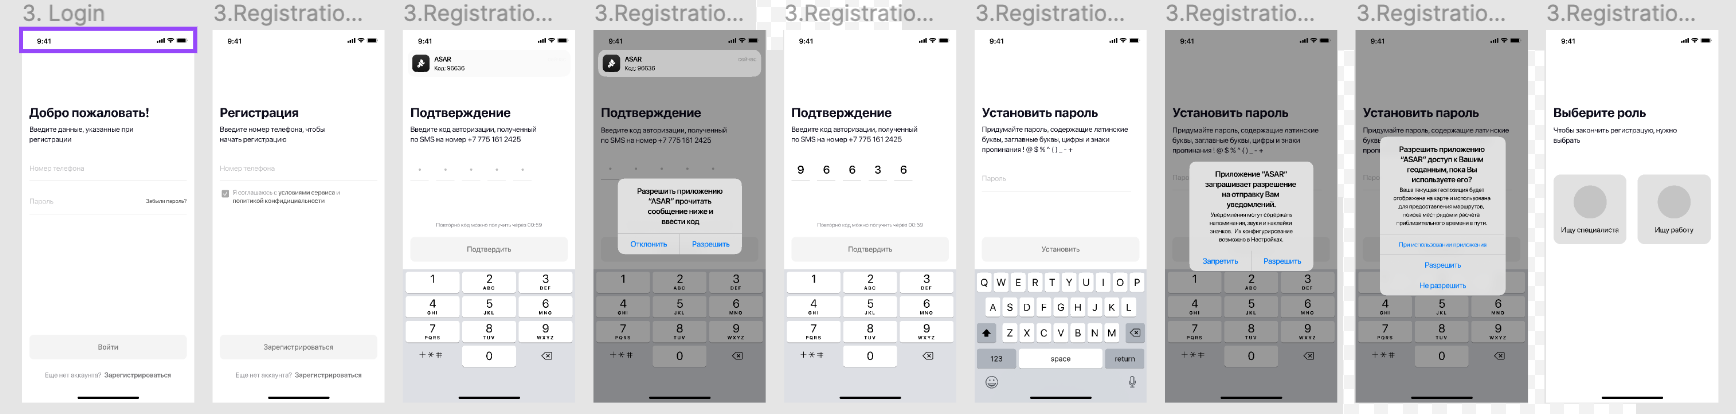
\includegraphics[scale=0.53]{images/design1.png}
\end{figure}
UX design of main page:
\begin{figure}[H]
    \centering
    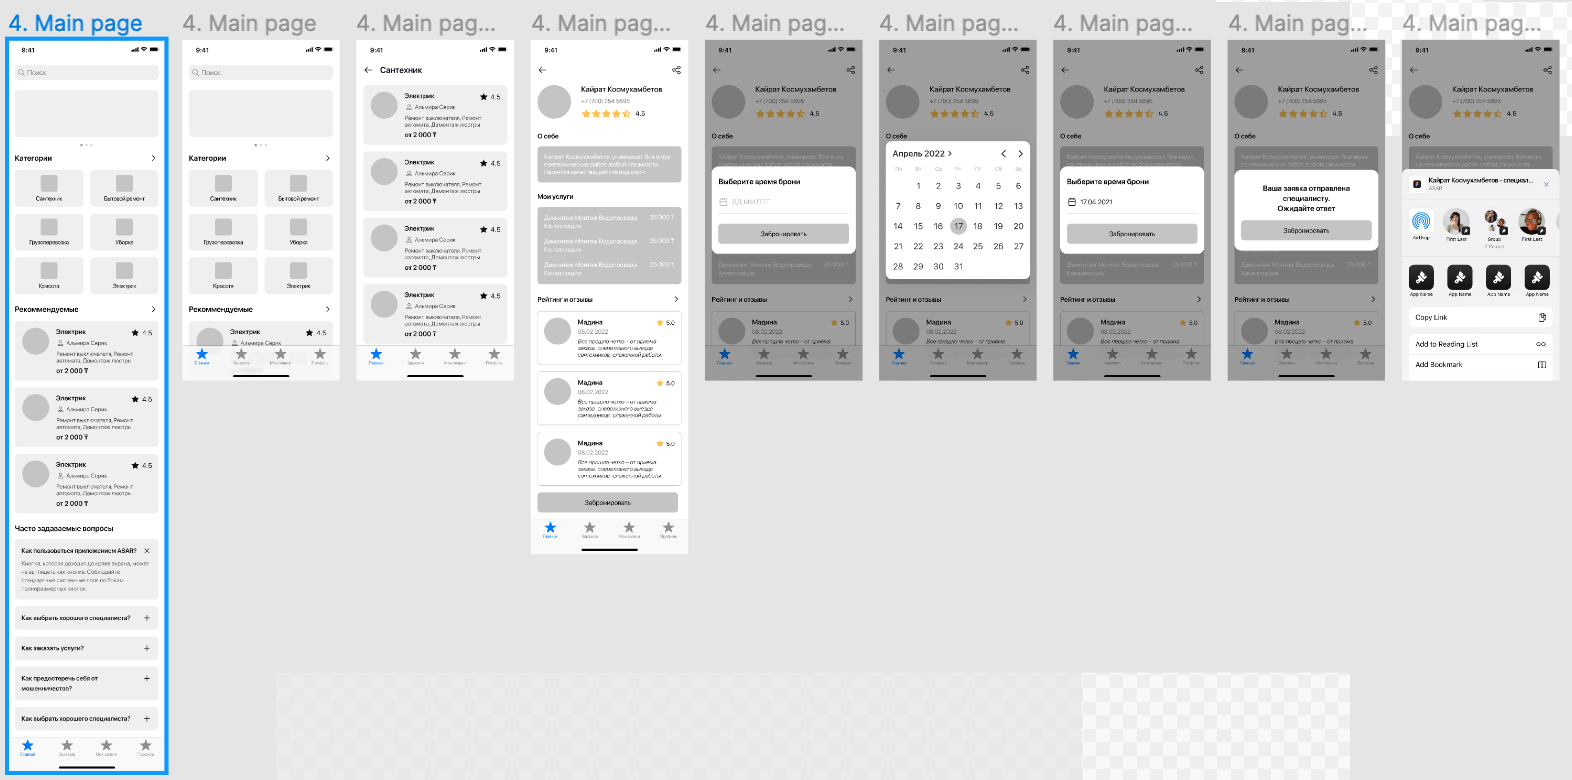
\includegraphics[scale=0.59]{images/design3.png}
\end{figure}
Ux design of creating orders and my orders:
\begin{figure}[H]
    \centering
    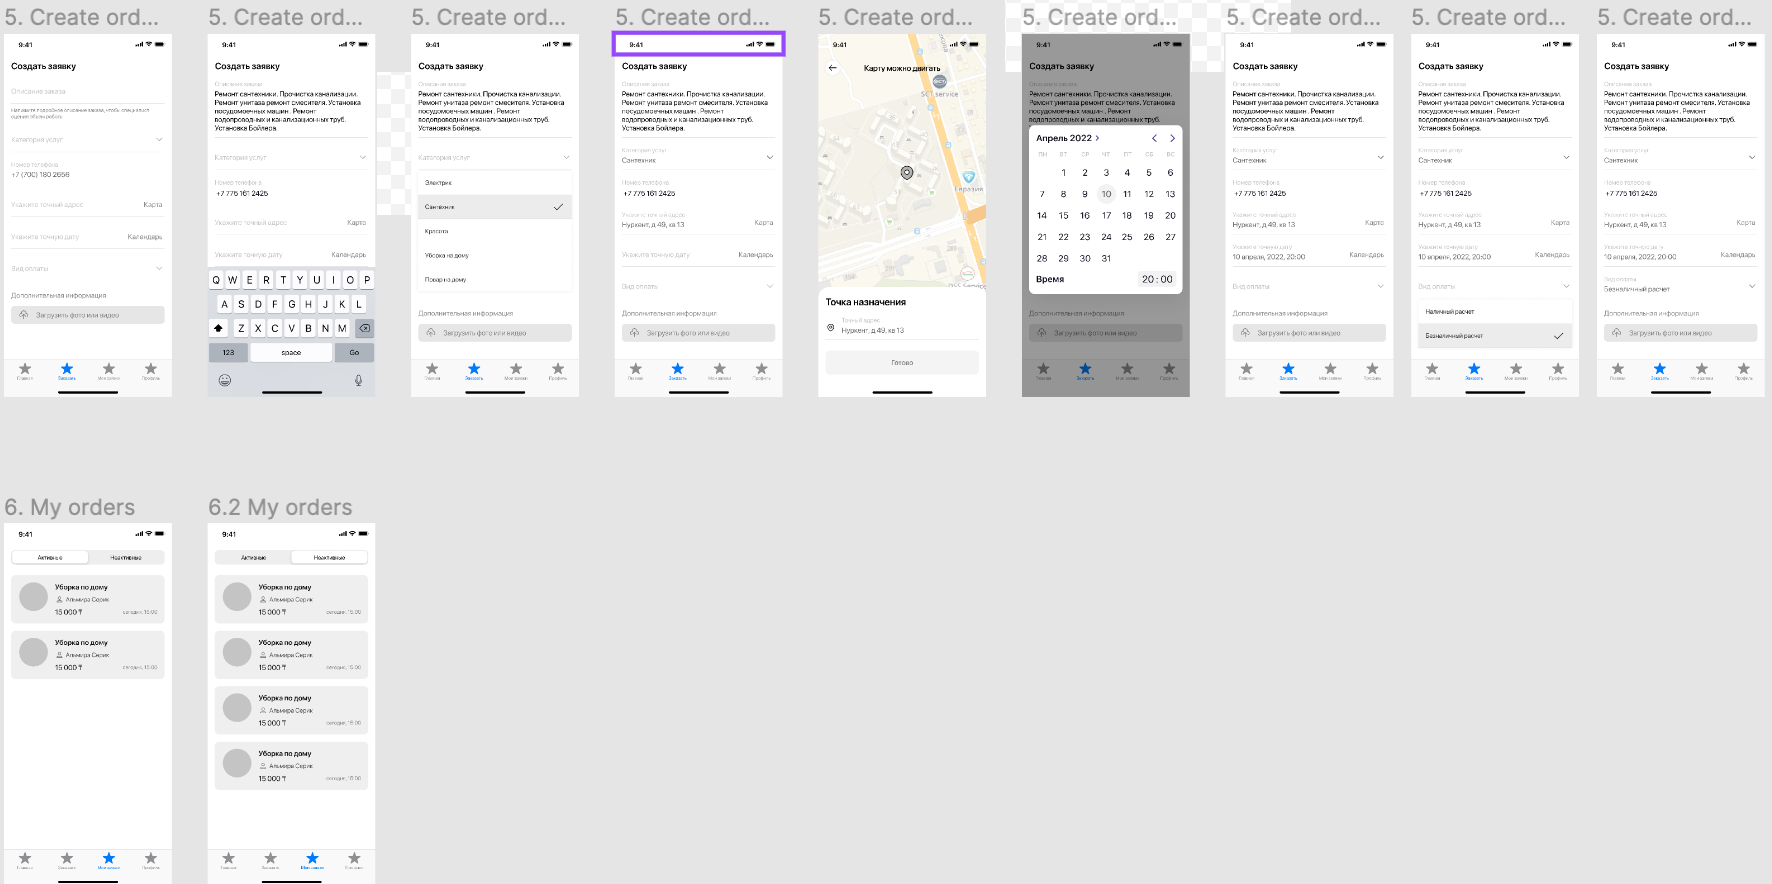
\includegraphics[scale=0.53]{images/design4.png}
\end{figure}
Next step was creating the User interface design part of our application, separately for clients and specialists flows. \newline
Registration and main page of client’s UI:
\begin{figure}[H]
    \centering
    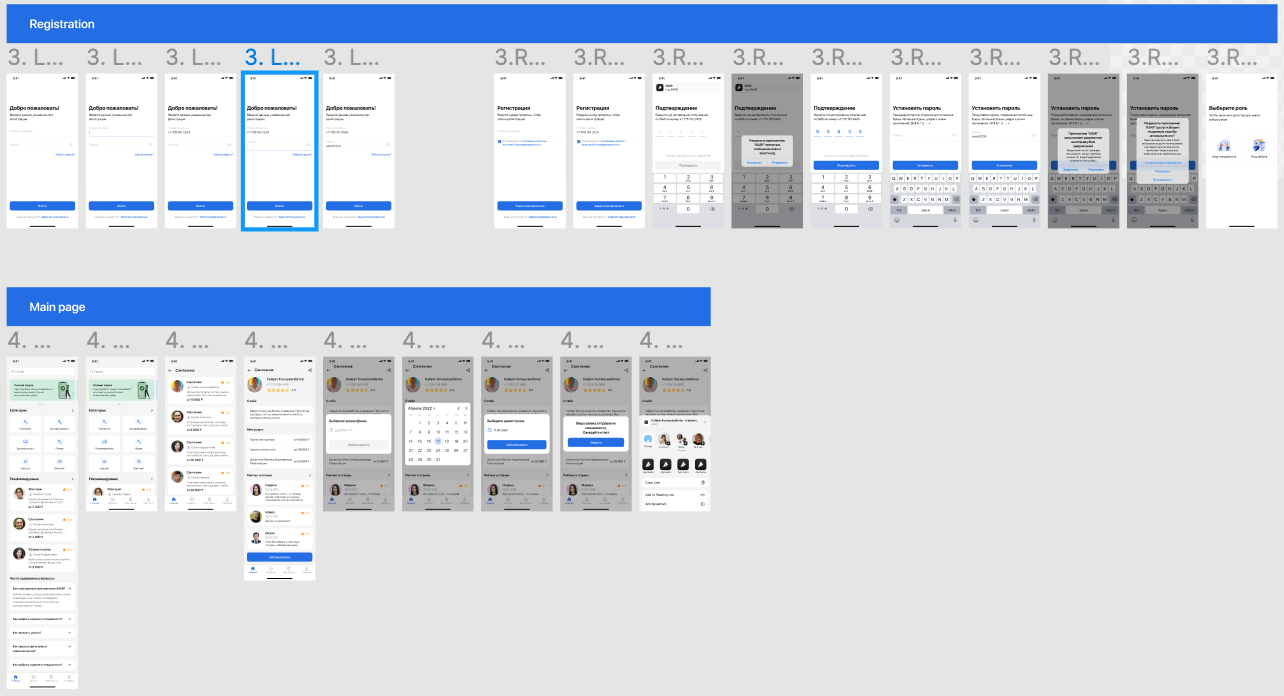
\includegraphics[scale=0.75]{images/design6.png}
\end{figure}
Create order and profile page of client’s UI:
\begin{figure}[H]
    \centering
    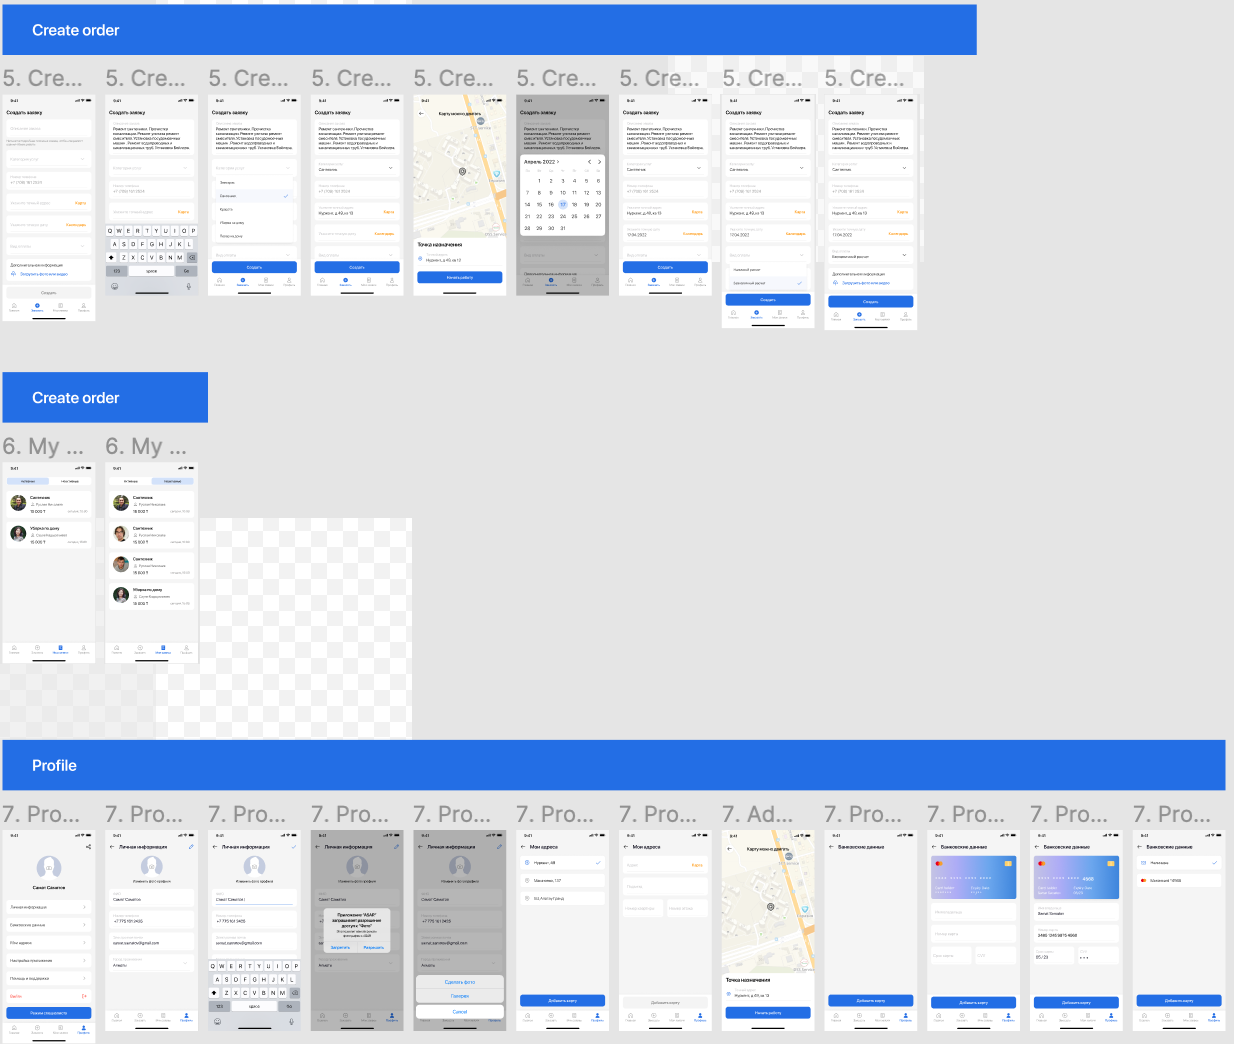
\includegraphics[scale=0.75]{images/design7.png}
\end{figure}
Specialist’s onboarding UI:
\begin{figure}[H]
    \centering
    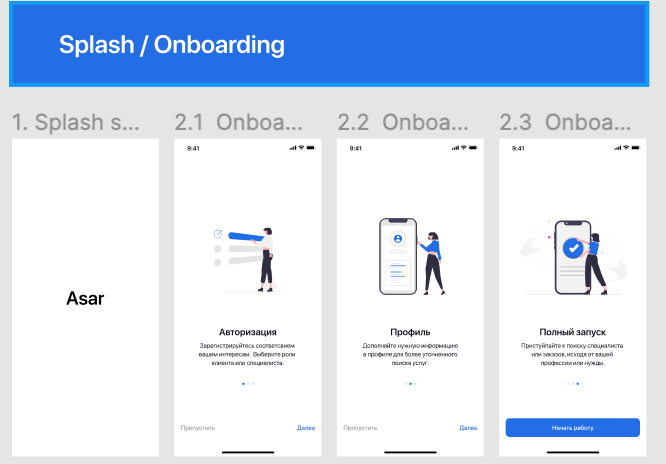
\includegraphics[scale=1.4]{images/design8.png}
\end{figure}
Registration page specialist’s UI:
\begin{figure}[H]
    \centering
    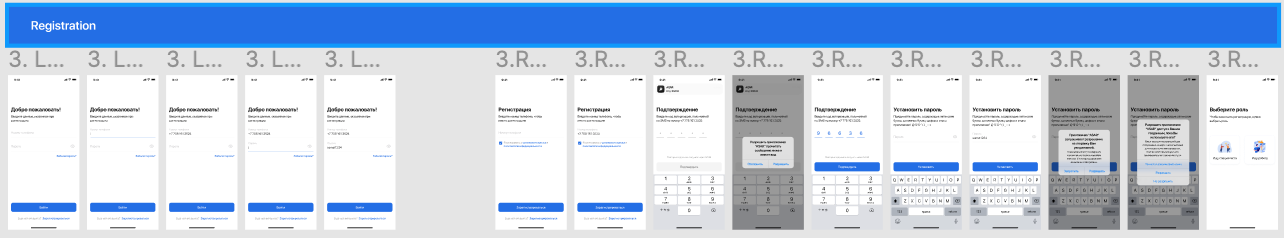
\includegraphics[scale=0.73]{images/design9.png}
\end{figure}
Main page UI:
\begin{figure}[H]
    \centering
    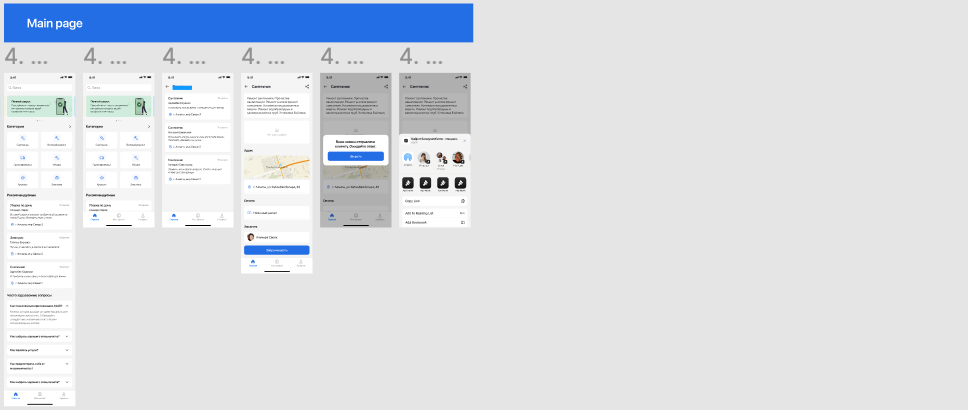
\includegraphics[scale=0.96]{images/design11.png}
\end{figure}
My orders and profile page:
\begin{figure}[H]
    \centering
    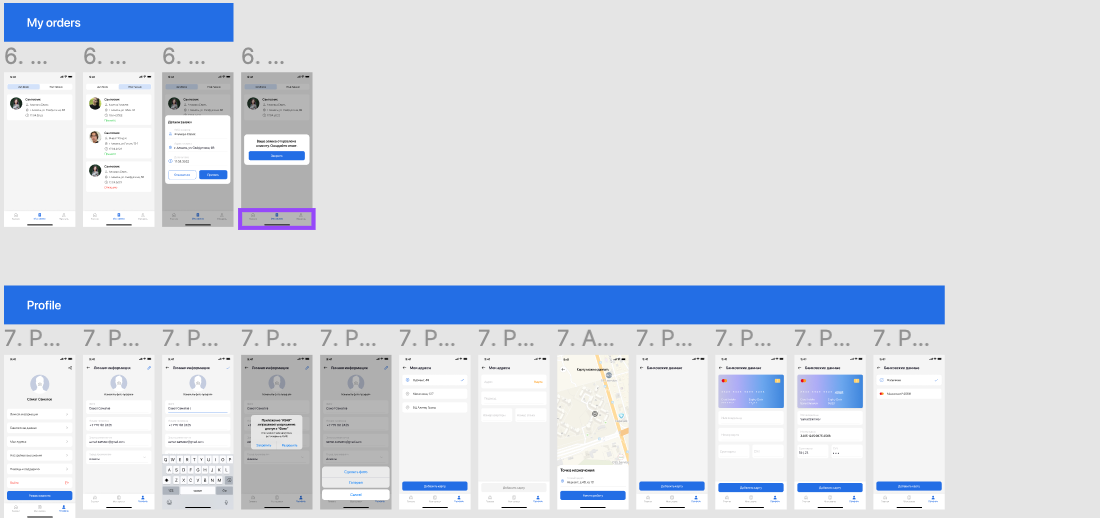
\includegraphics[scale=0.85]{images/design12.png}
\end{figure}
\section{Software for company clients and specialists}
\hspace{7mm}Explain the functionality of each flow, how many activities they have and what they do.
\subsection{Functionality for clients}
\hspace{7mm}If a user enters the application, until the registration all activities will be forbidden, except for onboarding cards. In the end of registration the user has the choice to be a client or to be a specialist.
\begin{figure}[H]
    \centering
    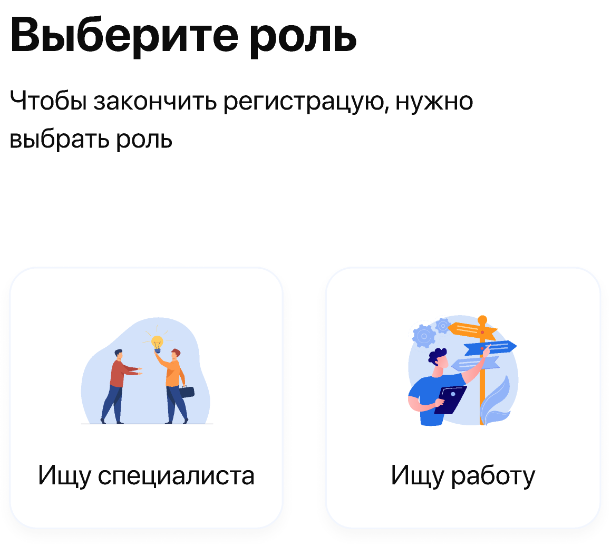
\includegraphics[scale=0.85]{images/func1.png}
\end{figure}
\hspace{-0.5cm}Following selection client, user will be able to have access to mobile application:
\begin{itemize}
    \item Search specialists by category
    \item See specialist’s personal information
    \item Book a specialist
    \item Create new order
    \item Edit profile page
    \item Change accessibility of options in settings
\end{itemize}


After authentication/registration, the user goes to the main page, there is a menu bar in the bottom, which are ‘Main Page’, ‘Order’, ‘My orders’, ‘Profile’.
\begin{figure}[H]
    \centering
    
\includegraphics[scale=0.55]{images/func2.png}
\end{figure}
On the ‘Main page’ of the application there are specialists by category. By clicking each of them, they can get short descriptions, prices, and reviews of people.
\begin{figure}[H]
    \centering
    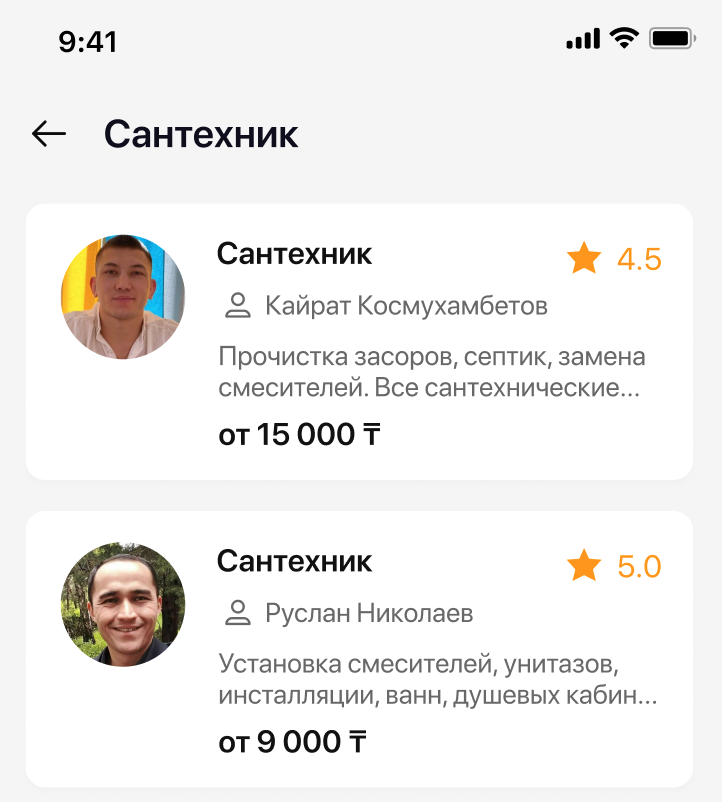
\includegraphics[scale=0.55]{images/func3.png}
    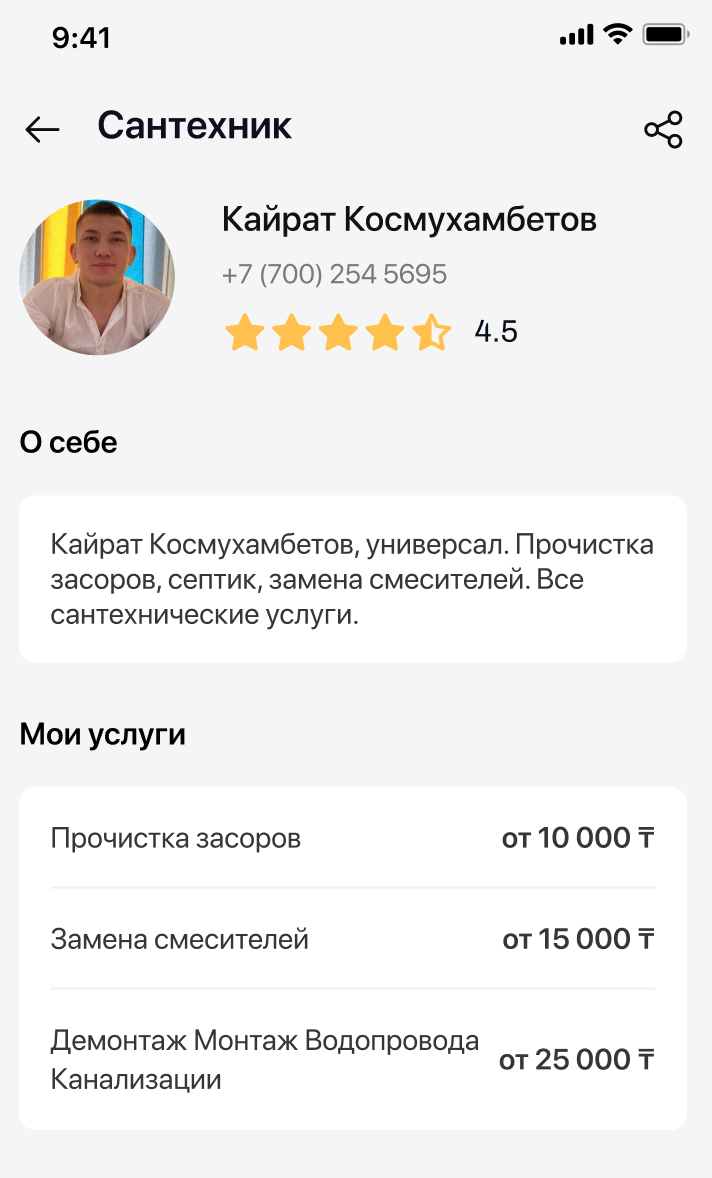
\includegraphics[scale=0.55]{images/func4.png}
\end{figure}
Also, there is a button ‘Book’, if they click it, it will give a modal with the date when they want to book them.
\begin{figure}[H]
    \centering
    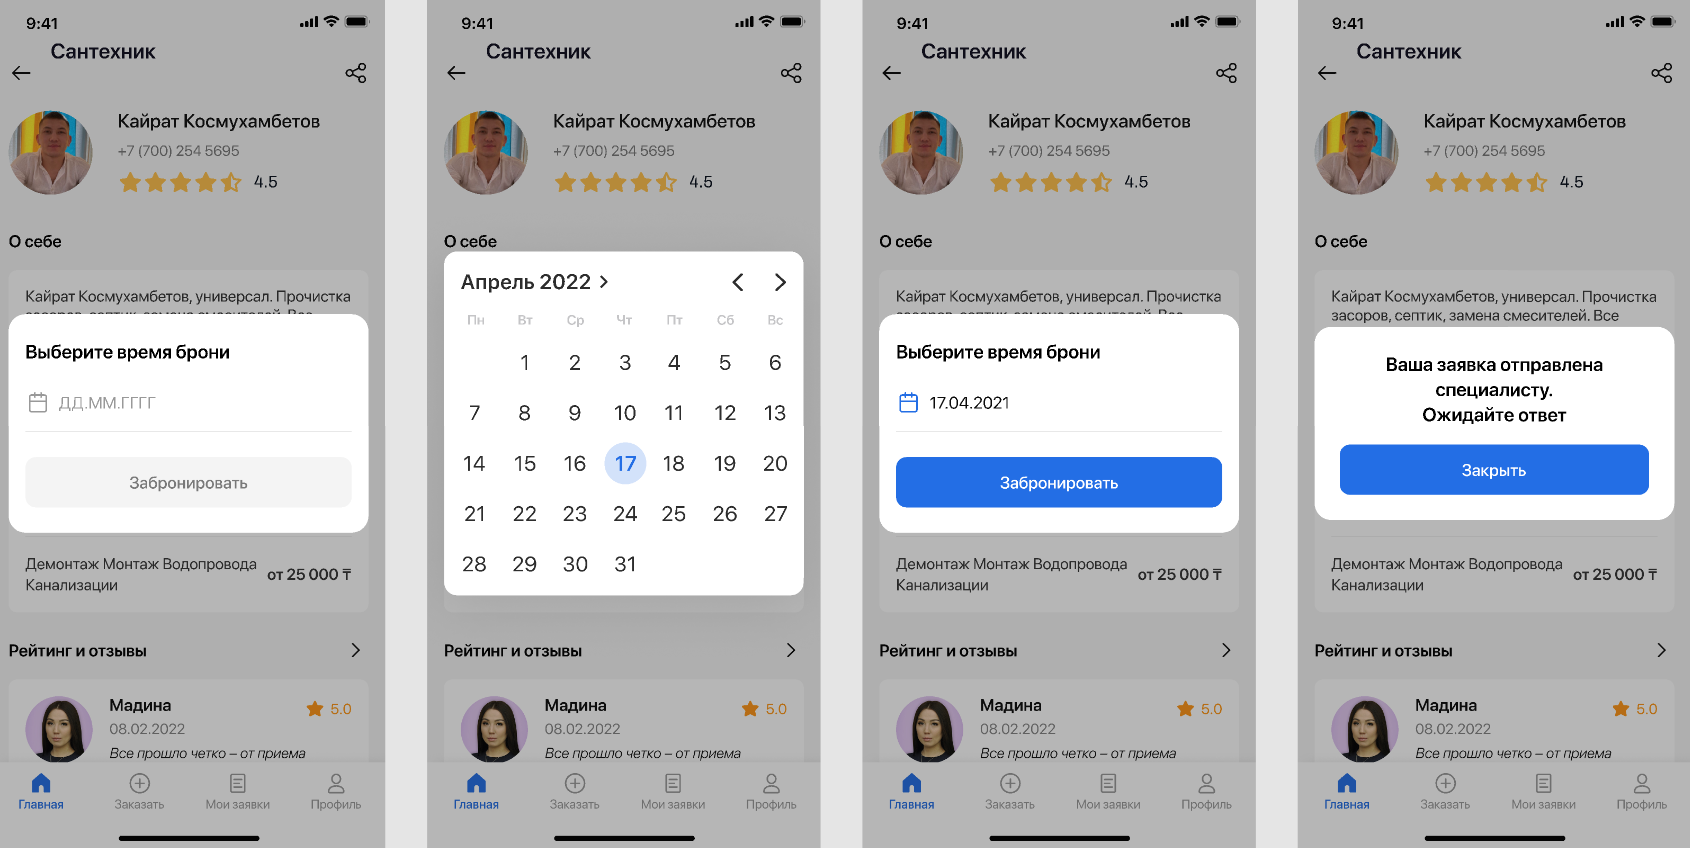
\includegraphics[scale=0.55]{images/func5.png}
\end{figure}
On the ‘Order’ page, users can create an order filling out the required data, such as description of service, address, date, payment type and others. On the ‘My orders’ users can see existing orders, and active or not.
\begin{figure}[H]
    \centering
    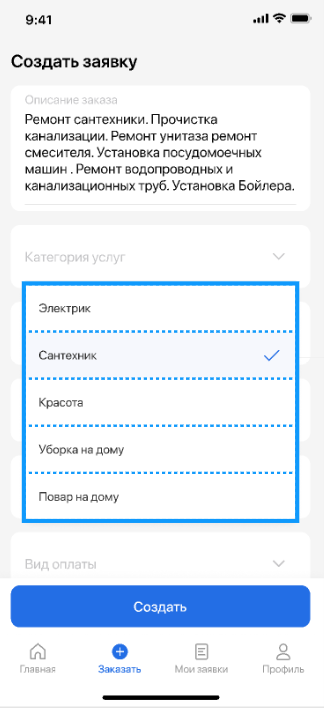
\includegraphics[scale=0.75]{images/func6.png}
    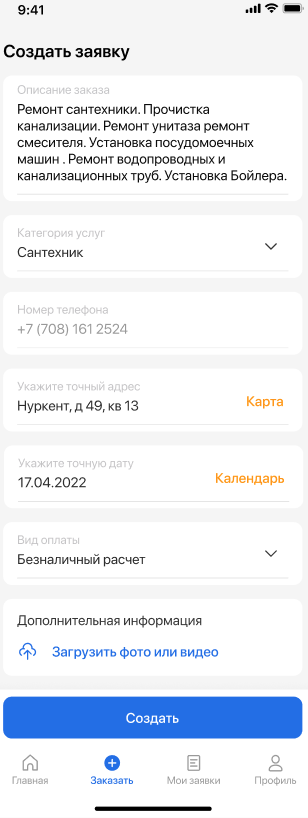
\includegraphics[scale=0.70]{images/func7.png}
\end{figure}
On the ‘Profile’ page users get six labels like: Personal information, Bank data, Address, Settings, Help and support, Logout. Users have the opportunity to easily edit information about themselves, bank data and addresses. Help and Support notificate them, how to use the app, privacy and security.
\subsection{Functionality for specialists}
\hspace{10mm}If users in the completing registration will choose specialist flow, all activities will be the same as the client's flow, except that the menu bar will differ.
\begin{figure}[H]
    \centering
    
\includegraphics[scale=0.75]{images/func8.png}
\end{figure}
On the ‘Main Page’ specialists can see categories of services and if they go through them, get the list of orders created by clients. Have the opportunity to click each of them, take a description of the service and press ‘Book’ to react. On the ‘My orders’ page there is a list of orders that specialists have taken, where orders are shown by their statuses.
\begin{figure}[H]
    \centering
    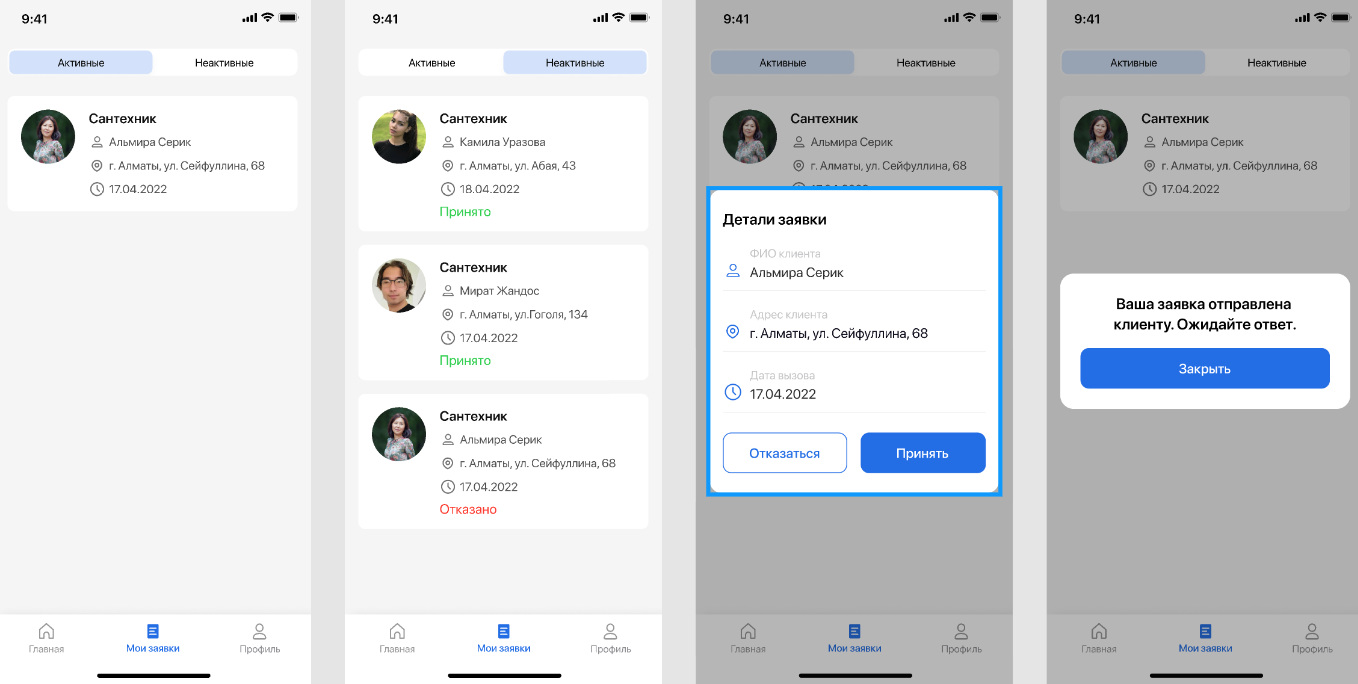
\includegraphics[scale=0.65]{images/func9.png}
\end{figure}
\section{Back-end}
\hspace{7mm}The back-end for this project was implemented in firebase. There is the easiest way to make authentication, password change, password reset, sms verification and so on. As well, firebase saved all images and data that were used in mobile application.
\begin{figure}[H]
    \centering
    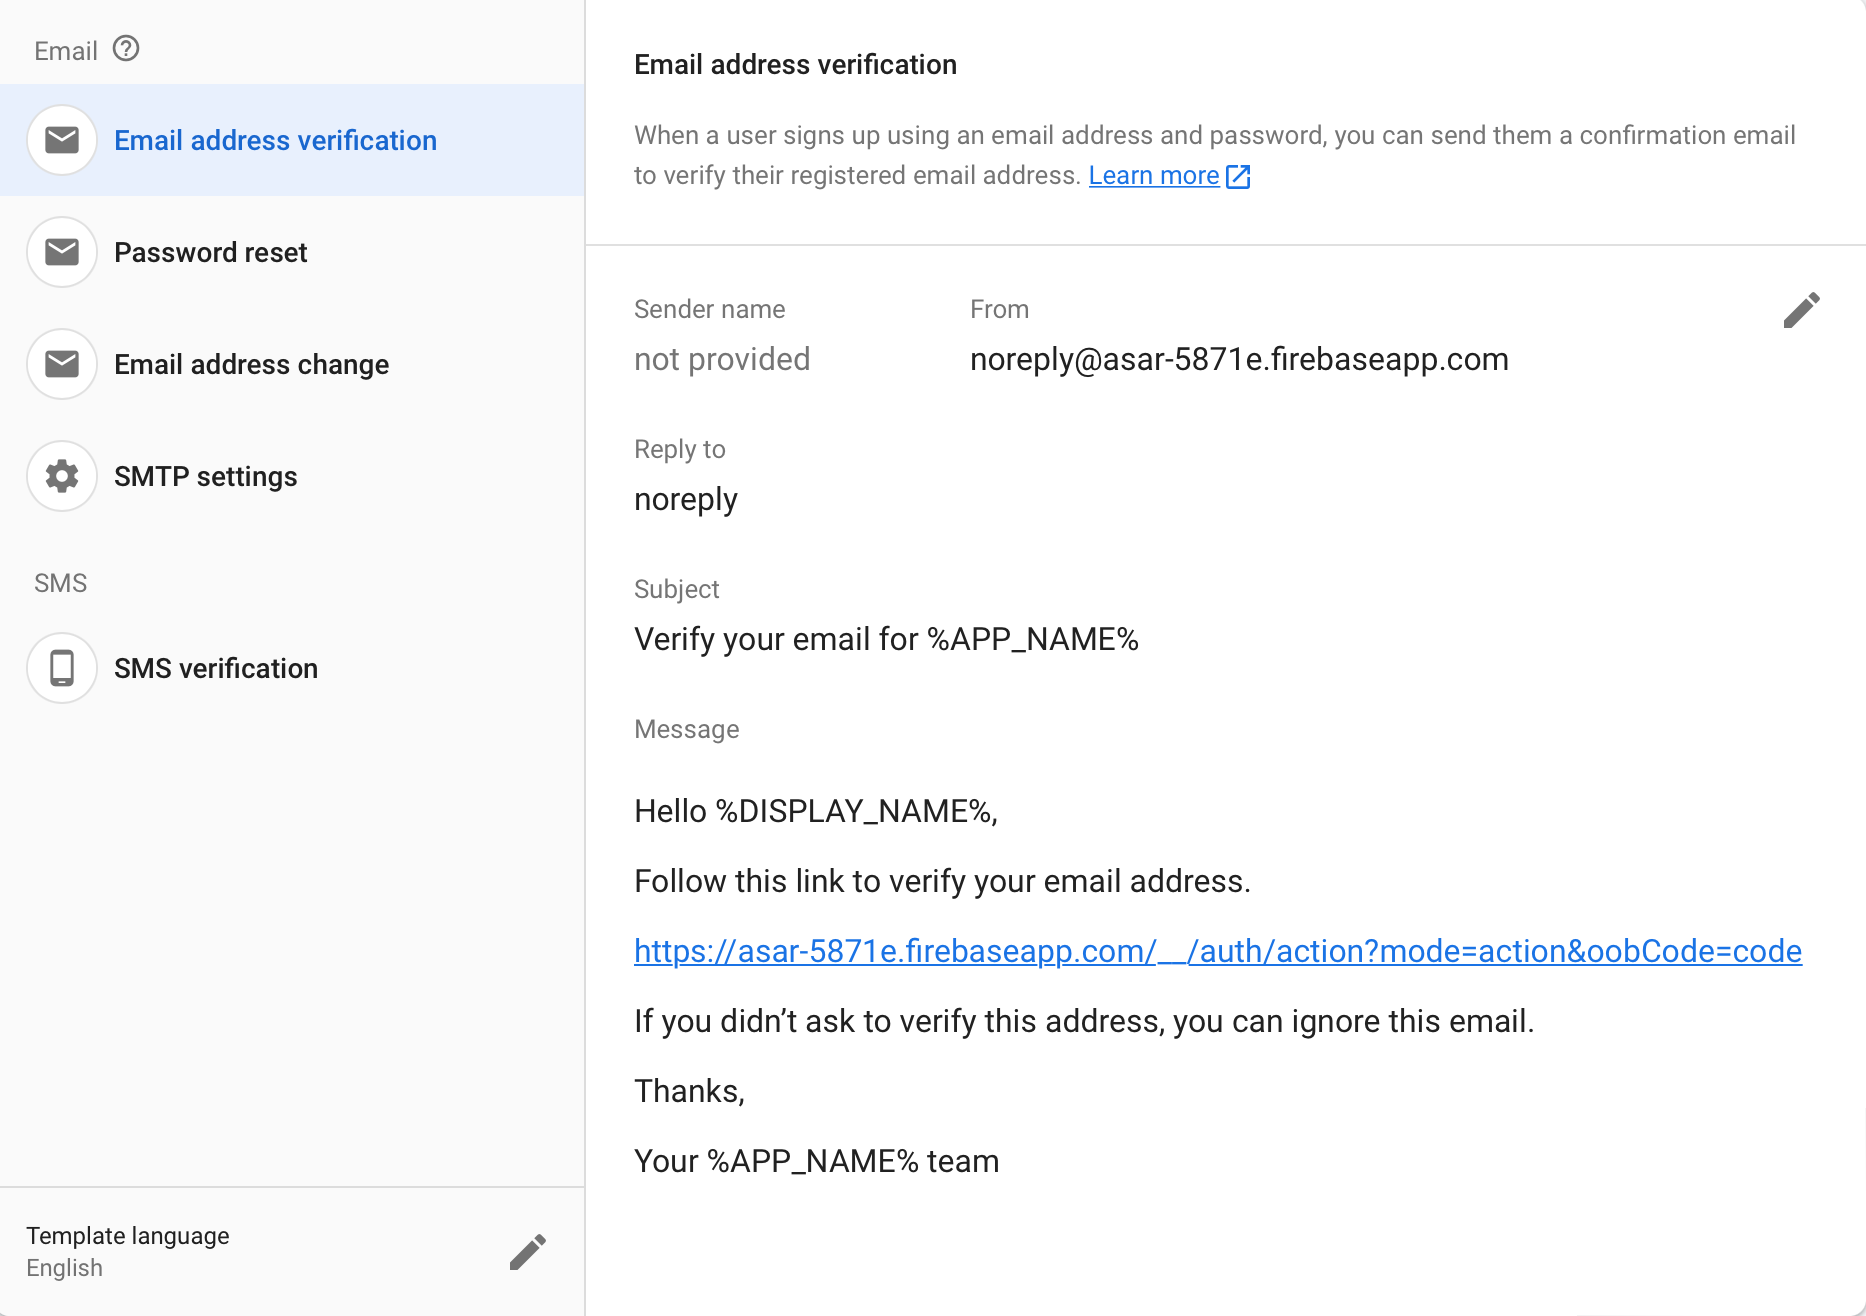
\includegraphics[scale=0.51]{images/back1.png}
\end{figure}
